%% LaTeX2e class for student theses
%% sections/evaluation.tex
%% 
%% Karlsruhe Institute of Technology
%% Institute for Program Structures and Data Organization
%% Chair for Software Design and Quality (SDQ)
%%
%% Dr.-Ing. Erik Burger
%% burger@kit.edu
%%
%% Version 1.3.5, 2020-06-26

\chapter{Evaluation}
\label{ch:Evaluation}

This chapter will focus on the performance evaluation of our novel SAT solver architecture. First we will talk about how the different benchmarks for this evaluation were created. Then we will look at how our SAT solver performs in comparison to other modern state of the art SAT solvers.

\section{Benchmarks}

In order to assess how good our novel SAT solver architecture performs, it is important to chose the correct benchmarks. Similar to other modern SAT solvers, our solver is capable of solving formulas that are represented as a CNF in a DIMACS file. Because SAT solving has a long history, there are a large amount of CNF benchmarks that can be used for a comparison in this area. While this evaluation will also contain performance comparisons on these CNF benchmarks, it isn't the focus of this thesis. As already described, this thesis tries to investigate if the structure of AMO and DNF constraints can be leveraged in order to gain an advantage compared to pure CNF solving. That's why our comparison is mostly focused on how fast our solver can solve benchmarks that contain these new constraints, compared to how fast other modern SAT solvers can solve the pure CNF equivalents. So in order to make this comparison possible, we implemented a program that converts benchmarks with AMO and DNF constraints to equivalent formulas in their CNF form.

\section{Encoding of AMO constraints}

Other modern SAT solvers were always capable of solving formulas that contained AMO and DNF constraints indirectly. Instead of supporting them natively, like our SAT solver, they just used an encoding in order to represent these constraints as a CNF. So in order to convert our benchmarks to their CNF equivalents, we just have to encode every AMO and DNF constraint. This isn't a simple task because there are many different encodings that have different strengths.

\paragraph{AMO constraints with a single literal}

This case is very simple, because AMO constraints that only contain a single literal, are actually always satisfied. An AMO constraint is satisfied if and only if at most one of its literals are true. Because it only contains a single literal, there can only ever be at most one literal that is true. This constraint is therefore redundant and can actually be removed

\paragraph{AMO constraints with less than six literals}

It was shown (find a source??) that for AMO constraints with less than six literals, the naive pairwise encoding hast the best performance.

\begin{figure}[h!t]
\label{form:pairwiseAMO}
\centering
\begin{leftbar}
\begin{displaymath}
AMO(x_1,...,x_n) = \bigwedge_{i=1}^{n - 1} \bigwedge_{j=i+1}^{n} \neg x_i \vee \neg x_j
\end{displaymath}
\end{leftbar}
\caption{Pairwise AMO encoding}
\end{figure}

Formula \ref{form:pairwiseAMO} shows the pairwise AMO encoding that is used for AMO constraints with less than six literals. The following example shows an AMO constraint with three literals and its CNF equivalent:

\begin{leftbar}
\begin{displaymath}
AMO(a,b,\neg c) \rightarrow (\neg a \vee \neg b) \wedge (\neg a \vee c) \wedge (\neg b \vee c)
\end{displaymath}
\end{leftbar}

\paragraph{AMO constraints with six or more literals}

For AMO constraints with six or more literals it is more efficient to use the sequential encoding which was introduced in the paper "Towards an Optimal CNF Encoding of
Boolean Cardinality Constraints" \cite{sinz2005towards} by Carsten Sinz. For AMO constraints with n literals it produces an encoding with 3n-4 clauses and n - 1 encoding variables \cite{sinz2005towards}.

\begin{figure}[h!t]
\label{form:sequentialAMO}
\centering
\begin{leftbar}
\begin{displaymath}
AMO(x_1,...,x_n) = (\neg x_1 \vee s_{1,1}) \wedge (\neg x_n \vee \neg s_{n-1,1}) \bigwedge_{1 < i < n} ((\neg x_i \vee s_{i,1}) \wedge (\neg s_{i-1,1} \vee s_{i,1}) \wedge (\neg x_i \vee \neg s_{i-1,1}))
\end{displaymath}
\end{leftbar}
\caption{Sequential AMO encoding \cite{sinz2005towards}}
\end{figure}

Formula \ref{form:sequentialAMO} shows the sequential encoding for AMO constraints. The following example shows how the encoding looks on a practical example:

\begin{leftbar}
\begin{displaymath}
AMO(a,b,\neg c) \rightarrow (\neg a \vee e) \wedge (c \vee f) \wedge (\neg b \vee f) \wedge (\neg e \vee f) \wedge (\neg b \vee \neg e)
\end{displaymath}
\end{leftbar}

Keep in mind that this example shows a sequential encoding for an AMO constraint with three literals. This is just to show how the encoding works. In our evaluation this encoding is only applied to AMO constraints with at least six literals.

\section{Randomized benchmarks}

Because the are no known sets of benchmarks that contain both AMO and DNF constraints in the form that our SAT solver needs, we needed to create our own benchmarks. One of the fastest ways to create benchmarks is a random generator. This has the advantage that it is possible to create very large sets of benchmarks in a short amount of time. But the randomization also makes it hard to control the difficulty of the benchmark. In order to make an accurate assessment on how good our SAT solver performs, we need benchmarks that are hard to solve. The randomization only allows us to control the number of variables, how many variables each constraint contains and how many constraints of each type are in the created formula.

In order to create hard 3-SAT instances it was shown that there occurs a phase transition at a variable to clause ratio of about 4.3 \cite{gent1994sat}. At this ratio about 50\% of the randomized 3-SAT instances are satisfiable. This ratio has a crossover with the point where very hard 3-SAT instances are created by the randomizer. So in order to create hard instances that contain other types of constraints, we decided to investigate if there exists a similar phase transition point for the other constraint types in our solver.

\subsection{Phase transition of AMO constraints}

\begin{figure}
\centering
  \begin{tikzpicture}[>=latex, scale=0.8]
\centering
\begin{axis}[
  axis x line=center,
  axis y line=center,
  width={\linewidth},
  xtick={0.01,0.02,...,0.09},
  ytick={0.1,0.2,...,1},
  xlabel={x},
  ylabel={y},
  xlabel style={below right},
  ylabel style={above left},
  xmin= 0,
  xmax=0.095,
  ymin=0,
  ymax=1.05]

  \addplot+ [mark=*] table {
0.0002 1.0
0.0052 1.0
0.0102 1.0
0.0152 0.999
0.0202 1.0
0.0252 0.99
0.0302 0.998
0.0352 0.992
0.0402 0.968
0.0452 0.924
0.0502 0.847
0.0552 0.63
0.0602 0.348
0.0652 0.127
0.0702 0.017
0.0752 0.001
0.0802 0.0

};

  \addplot+ [mark=*] table {
0.0002 0.132
0.0052 0.221
0.0102 0.332
0.0152 0.439
0.0202 0.530
0.0252 0.632
0.0302 0.743
0.0352 0.837
0.0402 0.926
0.0452 0.985
0.0502 1.0
0.0552 0.848
0.0602 0.552
0.0652 0.275
0.0702 0.109
0.0752 0.077
0.0802 0.069

};
\end{axis}

\end{tikzpicture}
\caption{Phase transition of AMO constraints with 7 literals}
\end{figure}

\begin{figure}
\centering
  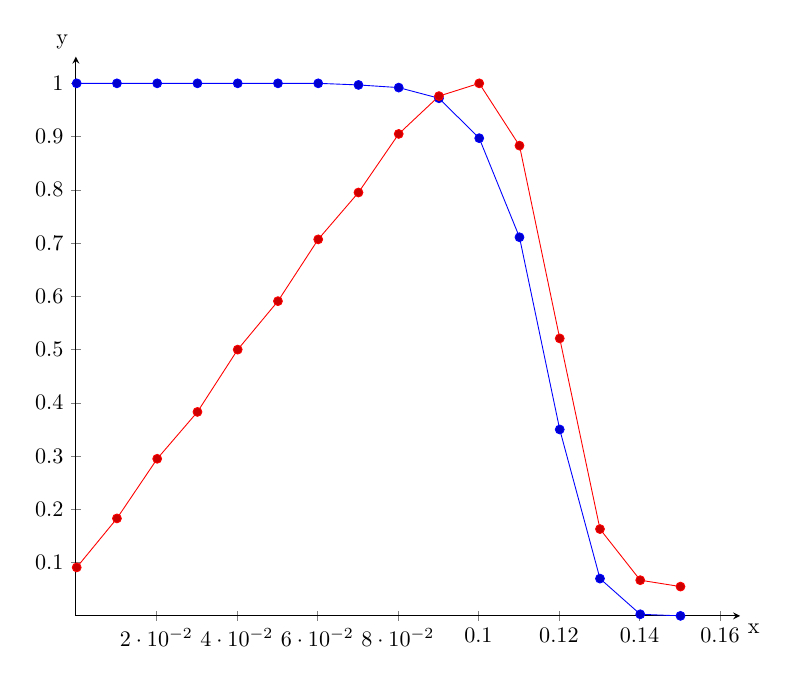
\begin{tikzpicture}[>=latex, scale=0.8]
\centering
\begin{axis}[
  axis x line=center,
  axis y line=center,
  width={\linewidth},
  xtick={0.02,0.04,...,0.16},
  ytick={0.1,0.2,...,1},
  xlabel={x},
  ylabel={y},
  xlabel style={below right},
  ylabel style={above left},
  xmin= 0,
  xmax=0.165,
  ymin=0,
  ymax=1.05]

  \addplot+ [mark=*] table {
0.0002 1.0
0.0102 1.0
0.0202 1.0
0.0302 1.0
0.0402 1.0
0.0502 1.0
0.0602 1.0
0.0702 0.997
0.0802 0.992
0.0902 0.972
0.1002 0.897
0.1102 0.711
0.1202 0.35
0.1302 0.07
0.1402 0.003
0.1502 0.0

};

  \addplot+ [mark=*] table {
0.0002 0.091
0.0102 0.183
0.0202 0.295
0.0302 0.383
0.0402 0.500
0.0502 0.591
0.0602 0.707
0.0702 0.795
0.0802 0.905
0.0902 0.976
0.1002 1.0
0.1102 0.883
0.1202 0.521
0.1302 0.163
0.1402 0.067
0.1502 0.055

};
\end{axis}

\end{tikzpicture}
\caption{Phase transition of AMO constraints with 5 literals}
\end{figure}


In order to estimate the phase transition of formulas with only AMO constraints, we experimented with several different setups. The first formula type contained only AMO constraints with five literals. The other formula type contained seven literals.

\subsection{Phase transition of DNF constraints}

Similar to the phase transition calculation for the AMO constraints, we also conducted experiments for formulas that only contain DNF constraints. Here we used DNF constraints with 5 terms that each contain 3 literals, DNF constraints with 3 terms that each contain 5 literals, and DNF constraints with 3 terms that each contain 3 literals.

\begin{figure}
\centering
  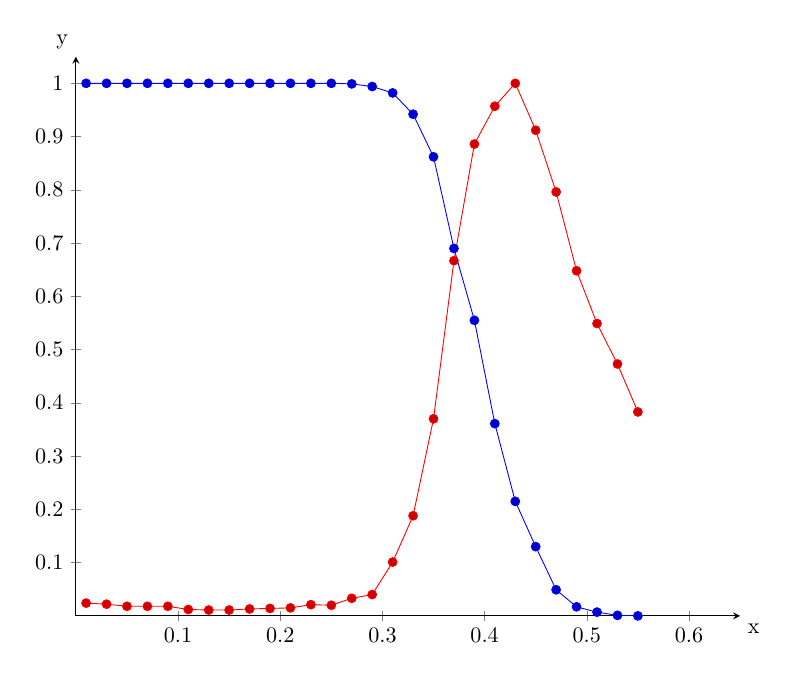
\begin{tikzpicture}[>=latex, scale=0.8]
\centering
\begin{axis}[
  axis x line=center,
  axis y line=center,
  width={\linewidth},
  xtick={0.1,0.2,...,0.6},
  ytick={0.1,0.2,...,1},
  xlabel={x},
  ylabel={y},
  xlabel style={below right},
  ylabel style={above left},
  xmin= 0,
  xmax=0.65,
  ymin=0,
  ymax=1.05]

  \addplot+ [mark=*] table {
0.01 1.0
0.03 1.0
0.05 1.0
0.07 1.0
0.09 1.0
0.11 1.0
0.13 1.0
0.15 1.0
0.17 1.0
0.19 1.0
0.21 1.0
0.23 1.0
0.25 1.0
0.27 0.999
0.29 0.994
0.31 0.982
0.33 0.942
0.35 0.862
0.37 0.69
0.39 0.555
0.41 0.361
0.43 0.215
0.45 0.13
0.47 0.049
0.49 0.017
0.51 0.007
0.53 0.001
0.55 0.0

};

  \addplot+ [mark=*] table {
0.01 0.024
0.03 0.022
0.05 0.018
0.07 0.018
0.09 0.018
0.11 0.012
0.13 0.011
0.15 0.011
0.17 0.013
0.19 0.014
0.21 0.015
0.23 0.021
0.25 0.020
0.27 0.033
0.29 0.040
0.31 0.101
0.33 0.188
0.35 0.370
0.37 0.667
0.39 0.886
0.41 0.957
0.43 1.0
0.45 0.912
0.47 0.796
0.49 0.648
0.51 0.549
0.53 0.473
0.55 0.383

};
\end{axis}

\end{tikzpicture}
\caption{Phase transition of DNF constraints with 3 terms of size 3}
\end{figure}

\begin{figure}
\centering
  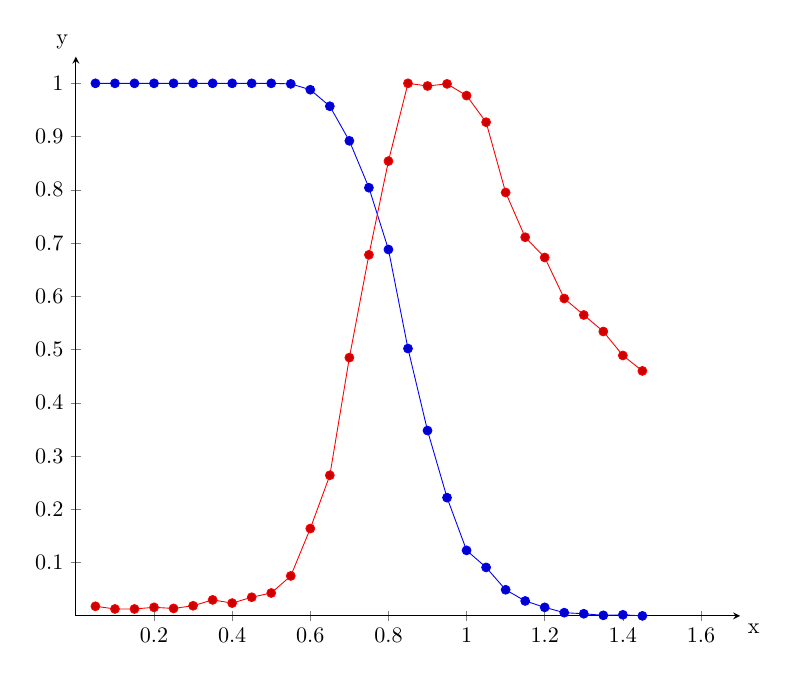
\begin{tikzpicture}[>=latex, scale=0.8]
\centering
\begin{axis}[
  axis x line=center,
  axis y line=center,
  width={\linewidth},
  xtick={0.2,0.4,...,1.6},
  ytick={0.1,0.2,...,1},
  xlabel={x},
  ylabel={y},
  xlabel style={below right},
  ylabel style={above left},
  xmin= 0,
  xmax=1.7,
  ymin=0,
  ymax=1.05]

  \addplot+ [mark=*] table {
0.05 1.0
0.1 1.0
0.15 1.0
0.2 1.0
0.25 1.0
0.3 1.0
0.35 1.0
0.4 1.0
0.45 1.0
0.5 1.0
0.55 0.999
0.6 0.988
0.65 0.957
0.7 0.892
0.75 0.804
0.8 0.688
0.85 0.502
0.9 0.348
0.95 0.222
1.0 0.123
1.05 0.091
1.1 0.049
1.15 0.028
1.2 0.016
1.25 0.006
1.3 0.004
1.35 0.001
1.4 0.002
1.45 0.0

};

  \addplot+ [mark=*] table {
0.05 0.018
0.1 0.013
0.15 0.013
0.2 0.016
0.25 0.014
0.3 0.019
0.35 0.03
0.4 0.024
0.45 0.035
0.5 0.043
0.55 0.075
0.6 0.164
0.65 0.264
0.7 0.485
0.75 0.678
0.8 0.854
0.85 1.0
0.9 0.995
0.95 0.999
1.0 0.977
1.05 0.927
1.1 0.795
1.15 0.711
1.2 0.673
1.25 0.596
1.3 0.565
1.35 0.534
1.4 0.489
1.45 0.46

};
\end{axis}

\end{tikzpicture}
\caption{Phase transition of DNF constraints with 5 terms of size 3}
\end{figure}
